\chapter{Projekt, etap I -- Badanie (Exploration)}
\label{cha:EtapI}

Zgodnie z cyklem życia ,,XP'' (więcej \namedref{sec:ZMTOcykl}), projekt zaczyna się od akwizycji ogólnego, głównego zadania systemu. Proponuje się w tym celu wykorzystać przygotowany szablon (więcej \namedref{sec:dodatekAsgzs}). Zawiera on nie tylko najważniejszą część, czyli ogólny opis głównego zadania systemu, ale także szereg pomocnych pytań pomagających w realizacji systemu zgodnie z oczekiwaniami klienta. Szablonu nie należy traktować jako idealnego, a raczej jako propozycję lub punkt wyjścia do rozwinięcia własnego dokumentu wykorzystywanego do akwizycji ogólnych wymagań w swoich projektach.

Sformułowanie głównego zadania systemu pozwala skupić się generowaniu kart wymagań związanych z~nim, a~nie ze~sprawami pobocznymi. Pozwala na uzmysłowienie grupie projektowej jaka jest główna część systemu wokół której należy się skupić.

\section{Specyfikacja wymagań}
\label{sec:EtapIsw}

\subsection{Specyfikacja głównego zadania systemu}
\label{sec:EtapIswSGZS}

Niżej przedstawiono szablon (więcej \namedref{sec:dodatekAsgzs}) wypełniony razem z klientem na jednym z pierwszych spotkań dotyczących wymagań systemu.

\begin{userstory}{Główne zadanie systemu}
Użytkownik za pomocą smartphone'a z kamerą działającego pod systemem Android lub za pomocą przeglądarki internetowej na komputerze stacjonarnym i kamery podłączonej do niego, ma możliwość udostępnienia on-line aktualnego obrazu i dźwięku.
    \begin{questions}
        \item{
            \textbf{Kto jest użytkownikiem systemu?} Użytkownikiem systemu może być każdy kto ma przeglądarkę. Aby udostępnić swoją kamerę dodatkowo użytkownik musi być zalogowany, a wcześniej zarejestrowany w systemie. Aby korzystać z reszty funkcji serwisu nie trzeba być zalogowanym.
        }
        \item{
            \textbf{Jakie urządzenia muszą współpracować z systemem?} Wszystkie komputery wyposażone w przeglądarkę IE 7.0+, Firefox 3+, Chrome, Opera 9+. Dodatkowo system ma działać na telefonach komórkowych / tabletach z systemem Android.
        }
        \item{
            \textbf{Czy jest wymóg użycia konkretnej technologii?} Nie jest wymagana żadna konkretna technologia. Wymaganiem jest wykorzystanie technologii Open Source -- wszędzie tam gdzie jesteśmy w stanie zastąpić komercyjne rozwiązania.
        }
        \item{
            \textbf{Jaka jest wymagana skalowalność systemu?} System musi być skalowalny, idealnie by było, gdyby obraz z kamery udostępniany przez jednego użytkownika, mógłby być odbierany przez nieskończoną liczbę ludzi. Na pewno w jakiś sposób system musi reagować automatycznie na zwiększony ruch w obrębie jednego stream'a.
        }
        \item{
            \textbf{Czy są jakieś wymagania dotyczące środowiska produkcyjnego w jakim ma działać system?} System docelowo będzie wdrożony na odpowiednim sprzęcie, testy powinien być w stanie odpalić się na średniej klasy laptopie. Im mniejsze wymagania tym lepiej.
        }
        \item{
            \textbf{Czy system ma współpracować z innymi systemami lub udostępniać coś innym systemom?} Duży nacisk będzie kładziony na integrację z serwisami społecznościowymi, głównie chodzi o Facebook'a. Będzie można go wykorzystać celem rejestracji i logowania w serwisie, czy też automatycznego udostępniania stream'u na swojej Facebook'owej ścianie.
        }
        \item{
            \textbf{Czy istnieją systemy podobne do tworzonego?} Jeżeli chodzi o sposób prezentacji interfejsu WWW to najbardziej zbliżony do tego co chce się osiągnąć jest Bambuser. Podobnie ma się sprawa funkcjonalności na telefonie z systemem Android -- aplikacja Bambuser.
        }
        \item{
            \textbf{Czy są jakieś inne specjalne wymagania, które nie wynikają z funkcji jakie powinien posiadać system (wymagania niefunkcjonalne)?} Szybki, skalowalny, bezpieczny, wykorzystujący technologie Open Source.
        }
    \end{questions}
\end{userstory}

\subsection{Karty wymagań dla ,,pierwszego wydania''}
\label{sec:EtapIswKWDPW}

Akwizycja głównego zadania systemu pozwala na przejście do kolejnego etapu, w którym przygotowuje się wszystkie karty wymagań dla ,,pierwszego wydania'' (więcej \namedref{sec:ZMTOcykl}). Faza ta trwa do momentu kiedy klient nie będzie już miał pomysłu na karty wymagań związane z głównym zadaniem systemu lub grupa projektowa nie będzie w stanie lepiej oszacować czasu potrzebnego na wykonanie danej karty wymagań bez rozpoczęcia jej implementacji.

\begin{userstory}{Strona główna dla niezalogowanego użytkownika}
    Użytkownikowi niezalogowanemu w systemie, po wejściu na główną domenę serwisu, zostaje zaprezentowana zawartość w postaci:
    \scr{img/strona_glowna.jpg}{Strona główna dla niezalogowanego użytkownika}
    \begin{packed_enum}
        \item odnośnik przekierowujący zawsze na stronę główną serwisu
        \item wyszukiwarka umożliwiająca wyszukiwanie udostępnionych streamów audio/video po kategoriach i lokalizacji
        \item dwa odnośniki, dzięki którym pokazuje się formularz logowania lub rejestracji
        \item mapa pokazująca grupy streamów audio/wideo
    \end{packed_enum}

    \begin{tests}
        \item{
            Użytkownik po wejściu na stronie główną widzi mapę swojej okolicy (fizycznej lokalizacji). Lokalizację możemy oszacować za pomocą IP lub jak jest taka możliwość w każdy inny dokładniejszy sposób.
        }
        \item{
            Użytkownik może dowolnie przesuwać mapą. Mapa reaguje na przesuwanie, oraz są na niej aktualizowane punkty streamów audio/video.
        }
    \end{tests}
\end{userstory}

\begin{userstory}{Strona główna dla zalogowanego użytkownika}
    Użytkownikowi zalogowanemu w systemie, po wejściu na główną domenę serwisu, zostaje zaprezentowana zawartość w postaci:
    \scr{img/strona_glowna2.jpg}{Strona główna dla zalogowanego użytkownika}
    \begin{packed_enum}
        \item avatar pobrany z gravatar.com oraz nazwa zalogowanego użytkownika
        \item wpis w menu przenoszący do podstrony ustawień zalogowanego użytkownika
        \item wpis w menu przenoszący do podstrony udostępniania streamu audio/video
    \end{packed_enum}
    \begin{tests}
        \item{
            Po kliknięciu w menu na pozycję z nazwą zalogowanego użytkownika, pojawiają się poniższe wpisy w menu.
        }
    \end{tests}
\end{userstory}

\begin{userstory}{Rejestracja}
    Użytkownik po naciśnięciu odnośnika rejestruj,
    zostaje przekierowany do formularza rejestracji:
    \scr{img/rejestracja.jpg}{Formularz rejestracji.}
    \begin{tests}
        \item{
            Pole email i powtórz email muszą być takie same, inaczej wyświetlany jest błąd, użytkownik proszony jest o poprawę pól.
        }
        \item{
            Pole hasło i powtórz hasło muszą być takie same, inaczej wyświetlany jest błąd, użytkownik proszony jest o poprawę pól.
        }
        \item{
            Pole loginu musi być unikalne w bazie. W przypadku wystąpienia w bazie zwracamy użytkownikowi błąd.
        }
        \item{
            Pole email musi być unikalne w bazie. W przypadku wystąpienia w bazie zwracamy użytkownikowi błąd.
        }
        \item{
            Po prawidłowym wypełnieniu formularza, użytkownik dostaje informację o konieczności potwierdzenia swojego adresu e-mail. Aby potwierdzić rejestrację musi kliknąć w link aktywacyjny wysłany na rejestrowane konto pocztowe, w ciągu 7 dni od momentu rejestracji. W innym wypadku konto nie zostanie aktywowane, a zgłoszenie usunięte z bazy.
        }
    \end{tests}
\end{userstory}

\begin{userstory}{Przypomnienie hasła}
    Użytkownik po naciśnięciu odnośnika zapomniałem hasła,
    zostaje przekierowany do formularza przypomnienia hasła:
    \scr{img/przypomnenie_hasla.jpg}{Formularz przypomnienia hasła.}
    \begin{tests}
        \item{
            Po wpisaniu istniejącego loginu lub maila, na maila wysyłane jest zapytanie, czy chcemy resetować hasło z linkiem aktywującym. Po jego kliknięciu otrzymujemy drugi mail z wygenerowanym nowym hasłem, które później możemy zmienić na zakładce ,,Ustawienia''.
        }
        \item{
            Użytkownik po podaniu błędnego loginu/maila zostaje o tym poinformowany ekranem:
            \scr{img/przypomnenie_hasla2.jpg}{Ekran informacji o błędnym wypełnieniu loginu/hasła.}
        }
    \end{tests}
\end{userstory}

\begin{userstory}{Logowanie użytkownika}
    Użytkownik po naciśnięciu odnośnika zaloguj,
    zostaje przekierowany do formularza logowania:
    \scr{img/logowanie.jpg}{Formularz logowania.}
    \begin{packed_enum}
        \item reszta strony wyszarzona, formularz logowania jako ,,overlay''
        \item klikając X'a wracamy do wyszarzonej strony
        \item miejsce na wpisanie loginu lub email
        \item miejsce na wpisanie hasła
        \item link do formularza przypomnienia hasła
        \item przycisk wysyłający formularz logowania
    \end{packed_enum}
    
    \begin{tests}
        \item{
            Użytkownik tylko po podaniu istniejącego loginu oraz pasującego do niego hasła
            zostaje zalogowany i przeniesiony na oglądaną przed logowaniem stronę.
        }
        \item{
            Użytkownik po zalogowaniu ma dostęp do dodatkowych podstron -- Ustawienia, Podziel się!
        }
        \item{
            Użytkownik po podaniu błędnego hasła lub nieistniejącego loginu, zostaje o tym poinformowany ekranem:
            \scr{img/logowanie2.jpg}{Ekran informacji o błędnym haśle lub loginie.}
            \begin{packed_enum}
                \item informacja o typie błędu
                \item oznaczenie pól jako błędnie wypełnionych, pole hasła pozostaje puste, pole loginu zostaje jako ostatnia wpisana wartość
            \end{packed_enum}
        }
        \item{Użytkownik po zalogowaniu widzi zmodyfikowane menu -- na wszystkich podstronach serwisu.}
        \scr{img/strona_glowna2.jpg}{Zmodyfikowane menu na górze}
    \end{tests}
\end{userstory}

\begin{userstory}{Udostępnianie streamu audio/video krok pierwszy}
    Użytkownik po wybraniu z menu opcji podziel się,
    zostaje przekierowany do formularza udostępniania audio/video:
    \scr{img/dzielenie_sie_streamem1.jpg}{Formularz udostępniania audio/video.}
    \begin{packed_enum}
        \item {Aby udostępnić stream należy wybrać kategorię, do której ten stream ma być przypisany. Lista kategorii jest przykładową lista, administrator ma mieć możliwość modyfikowania tej listy z poziomu panelu administracyjnego.}
        \item {Jeżeli w systemie istnieje więcej niż jedna kamera, tutaj wybierana jest kamera źródłowa. Domyślnie wybraną jest pierwsza systemowa kamera.}
        \item {Możemy wybrać jakość transmisji spośród:
            \begin{packed_item}
                \item{wysoka -- wysoka jakość z preferencją wideo nad audio}
                \item{średnia -- średnia jakość zarówno wideo jak audio}
                \item{niska -- niska jakość wideo z preferencją jakości audio nad wideo}
            \end{packed_item}
        }
        \item{Po kliknięciu ,,Podziel się'' na formularzu udostępniania audio/video, użytkownikowi otwiera się nowe okno przeglądarki gdzie prezentowane są dane udostępnionego streamu (krok drugi). W starym oknie użytkownik zostaje przekierowany do poprzednio odwiedzanej strony -- przed wybraniem ,,Podziel się''.}
        \item {Wybór dostępności streamu, albo publiczny -- wszyscy użytkownicy systemu mogą go oglądać/udostępniać (domyślna opcja) -- lub prywatny -- tylko posiadający link do streamu mogą go zobaczyć.}
    \end{packed_enum}
    \begin{tests}
        \item{Jeżeli w systemie nie ma kamery, użytkownik jest informowany o braku możliwości udostępniania, przycisk ,,Podziel się!'' staje się nieaktywny.}
    \end{tests}
\end{userstory}

\begin{userstory}{Udostępnianie streamu audio/video krok drugi}
    Po kliknięciu ,,Podziel się'' na formularzu udostępniania audio/video, użytkownikowi otwiera się nowe okno przeglądarki gdzie prezentowane są dane udostępnionego streamu. W starym oknie użytkownik zostaje przekierowany do poprzednio odwiedzanej strony -- przed wybraniem ,,Podziel się''.
    \scr{img/dzielenie_sie_streamem2.jpg}{Okno danych udostępnianego streamu audio/video.}
    \begin{packed_enum}
        \item{możliwość zmiany kamery oraz jakości w trakcie nadawania}
        \item{jeżeli wcześniej wybrano publiczną dostępność streamu, wyświetlamy tutaj unikalny link do dzielenia się streamem ze znajomymi np. za pomocą Facebook'a, w przeciwnym wypadku wyświetlamy ,,permalink'' streamu w formie \url{http://domena.com/login_usera/slug_tytulu_streamu}}
        \item{przycisk otwierający w nowym oknie link streamu}
        \item{informacja na temat tytułu oraz kategorii udostępnianego streamu}
    \end{packed_enum}
    \begin{tests}
        \item{Po kliknięciu na pole tekstowe linku, zaznacza się cała zawartość. Dodatkowo zaznaczona zawartość zostaje skopiowana do schowka, na ekranie pojawia się informacja ,,Link skopiowano do schowka!''}
    \end{tests}
\end{userstory}

\section{Analiza wymagań}
\label{sec:EtapIaw}

Po rozmowie z klientem, na podstawie ,,głównego zadania systemu'' oraz innych przygotowanych kart wymagań, można przejść do fazy analizy wymagań (więcej w \namedref{sec:ZMTOzwinnaAnalizaWymagan}).

Celem tego etapu jest stworzenie wstępnej architektury systemu, przetestowanie wydajności technologii -- najczęściej przy użyciu prototypu systemu.

Jako początek rozważań architektury systemu skorzystano z elementów metody Architecture Tradeoff Analysis Method -- ,,Drzewo użyteczności'' -- szczegóły metody można poznać w \cite{Kaz2000}.

Pełna metoda ATAM wprowadza zbyt dużą formalizację i generuje zbyt dużą ilość dokumentacji, z której metodyki zwinne chcą rezygnować. Dodatkowo zgodnie z założeniami ,,XP'' (więcej \namedref{sec:ZMTOzalozenia}), wszystkie ustalenia sporządzone w tej fazie mogą ulec zmianie na każdym późniejszym etapie prowadzenia projektu. Zwinna analiza wymagań nie zamyka możliwości późniejszej zmiany technologii, architektury czy dowolnego z elementów wspomagających projekt.

\subsection{Drzewo użyteczności (ATAM Usability Tree)}
\label{sec:EtapIdrzewoUzytecznosci}

\begin{packed_item}
    \item{
        \textbf{WYDAJNOŚĆ}
        \begin{packed_item}
            \item{
                Opóźnienie transmisji danych
                \begin{packed_item}
                    \item{opóźnienie wideo dostosowane do aktualnej przepustowości łącza, jak najmniejsze}
                    \item{brak lub minimalne opóźnienia transmisji audio}
                \end{packed_item}
            }
            \item{
                Ilość użytkowników
                \begin{packed_item}
                    \item{Liniowa zależność ilość użytkowników używających system od zużywanych zasobów}
                    \item{Minimalna ilość użytkowników aktywnie poruszających się po stronie -- 1000 osób}
                    \item{Minimalna ilość użytkowników oglądających jeden strumień wideo -- 100 osób}
                \end{packed_item}
            }
        \end{packed_item}
    }
    \item{
        \textbf{MODYFIKOWALNOŚĆ}
        \begin{packed_item}
            \item{Zarządzanie użytkownikami}
            \item{Zarządzanie dostępnymi streamami}
            \item{Zarządzanie kategoriami streamów}
            \item{Aktualizacja i dystrybucja oprogramowania mobilnego}
            \item{Łatwa modyfikacja wyglądu strony}
        \end{packed_item}
    }
    \item{
        \textbf{DOSTĘPNOŚĆ}
        \begin{packed_item}
            \item{Dostępność całej usługi na poziomie 99,9\% rocznie}
            \item{Dostępność usługi na urządzenia mobilne (tablety, telefony)}
            \item{Dostępność usługi na desktopy}
        \end{packed_item}
    }
    \item{
        \textbf{SKALOWALNOŚĆ}
        \begin{packed_item}
            \item{Odporność na geometryczną ,,nagłą popularyzację''}
            \item{Liniowa zależność ilość użytkowników/zużywane zasoby}
        \end{packed_item}
    }
    \item{
        \textbf{BEZPIECZEŃSTWO}
        \begin{packed_item}
            \item{
                System logowania
            }
            \item{
                Stream publiczny/prywatny
            }
            \item{
                Szyfrowanie
                \begin{packed_item}
                    \item{wymagane szyfrowanie transmisji wideo}
                    \item{wymagane szyfrowanie transmisji audio}
                    \item{wymagane szyfrowanie transmisji http i każdej innej transmisji danych poza system}
                \end{packed_item}
            }
        \end{packed_item}
    }
\end{packed_item}

\subsection{Wstępna architektura systemu}
\label{sec:EtapIwstepnaArchitekturaSystemu}

Docelowy system będzie się składał z \textbf{Interfejsu WWW}, odpowiedzialnego za prezentację mapy i dostosowywanie się do zmiennej szerokości ekranu urządzeń. Wszystkie stream'y będą umieszczone w relacyjnej \textbf{Bazie danych} z rozszerzeniem GIS, dzięki czemu możliwe będzie łatwe zapisanie lokalizacji stream'u.

Po stronie komputerów stacjonarnych, za pobieranie obrazu z kamery i wyświetlanie obrazu u drugiego użytkownika będzie odpowiedzialny obiekt SWF \textbf{Adobe Flash Player}. W przypadku urządzeń mobilnych, do przygotowania aplikacji obsługującej zarówno iPhone'a jak i Androida wykorzystany zostanie otwarty framework Adobe Flex i jego mobilne wsparcie w postaci \textbf{Adobe AIR for Mobile}.

Do rozproszenia ruchu i stworzenia systemu niezależnego od pojedynczego punktu połączenia sieciowego -- osoby udostępniającej stream -- będą wykorzystane sieci ze wspomaganiem równorzędnym wbudowane w Adobe Flash Platform. Zasada działania sieci P2P, wymusza udostępnianie oglądanego streamu, tak aby zapewnić prostą zależność -- im więcej użytkowników chce oglądać, tym więcej użytkowników udostępnia żądany stream. Firma Adobe nazywa tę technologię \textbf{Multicast/P2P Multicast}, niżej przedstawione są schematy pokazujące różnicę pomiędzy transmisją Unicast, a P2P Multicast. \footnote{informacje dotyczące technologii Adobe oraz obrazki zostały pobrane z \cite{TomKrcha2010ME} oraz \cite{MattKauf2009}}

\begin{center}
    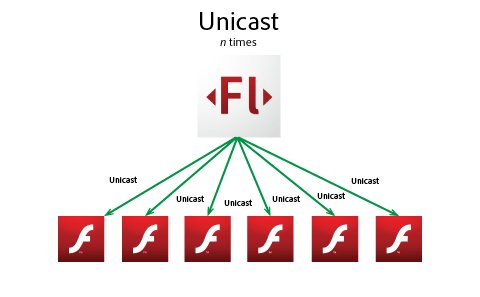
\includegraphics[width=\textwidth]{img/adobe-p2p-unicast.jpg}
    \captionof{figure}{Adobe Flash Platform Unicast -- wszystko zależne od przepustowości jednego elementu źródłowego, serwera plików}
\end{center}

\begin{center}
    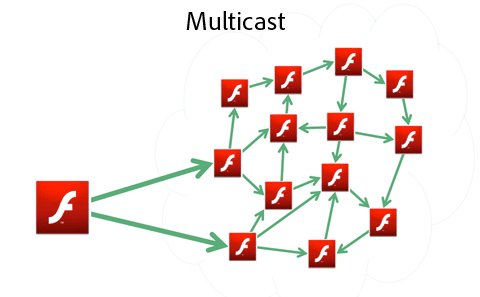
\includegraphics[width=\textwidth]{img/adobe-p2p-multicast.jpg}
    \captionof{figure}{Adobe Flash Platform P2P Multicast -- obciążenie rozłożone na całość sieci ze wspomaganiem równorzędnym}
\end{center}

\newpage
Jako, że część technologie, które zostaną wykorzystane są nowe dla całej ,,grupy projektowej'', będzie potrzebny prototyp systemu. Niżej przedstawiono schematy pokazujące powiązanie pomiędzy poszczególnymi elementami systemu:

\begin{center}
    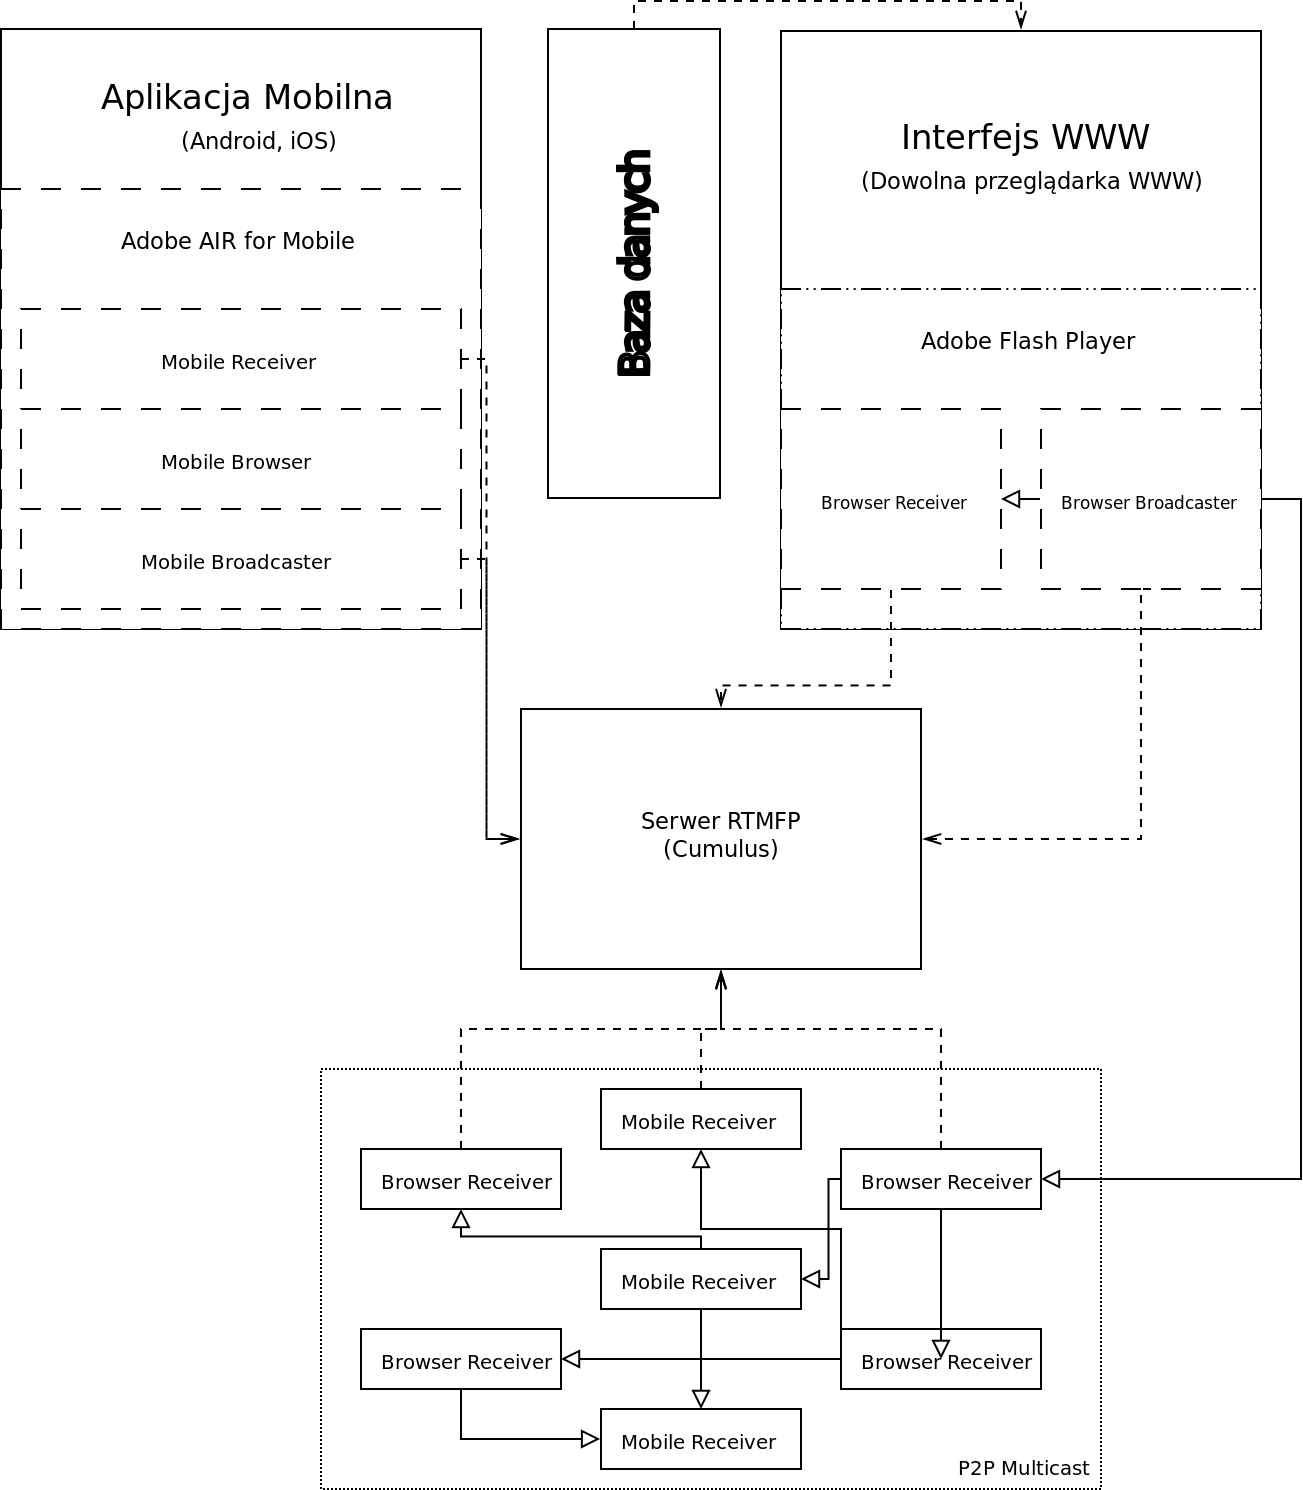
\includegraphics[width=\textwidth]{diagramy/architektura.png}
    \captionof{figure}{Wstępna architektura systemu.}
\end{center}

\begin{minipage}{\textwidth}
    \begin{description}
        \item[Interfejs WWW]{Centralny interfejs użytkownika z systemem, umożliwia przeglądanie stream'ów z poziomu przeglądarki WWW, implementuje design dostosowywany do szerokości ekranu urządzenia na którym się go przegląda. Współpracuje z wszystkimi nowoczesnymi przeglądarkami WWW. Udostępnia API do komunikacji z aplikacją mobilną czy samym obiektem SWF.}
        \item[Baza Danych]{Centralne miejsce składowania wszystkich danych przechowywanych w systemie. Umożliwia szybkie wyszukiwanie, jest bezpośrednio połączona z Interfejsem WWW, który przez swoje API udostępnia przechowywane przez nią dane.}
        \item[Browser Receiver]{Aplikacja Adobe Flash Player, umożliwiająca dołączenie do stream'u wideo nadawanego przez Browser Broadcaster lub Mobile Broadcaster.}
        \item[Browser Broadcaster]{Aplikacja Adobe Flash Player, umożliwiająca nadawanie stream'u wideo bezpośrednio z przeglądarki.}
        \item[Mobile Receiver]{Aplikacja mobilna Adobe AIR for Mobile, umożliwiająca odbieranie stream'u wideo nadawanego przez Mobile Broadcaster lub Browser Broadcaster z poziomu urządzenia wspierającego iOS lub Android'a.}
        \item[Mobile Broadcaster]{Aplikacja mobilna Adobe AIR for Mobile, umożliwiająca nadawanie stream'u wideo z poziomu urządzenia wspierającego iOS lub Android'a.}
        \item[Serwer RTMFP]{Serwer przechowujący informację na temat listy osób biorących udział w transmisji wideo stream'ów. Dzięki niemu pokonujemy niefiltrowany NAT. Łączą się z nim wszystkie aplikacje Broadcaster oraz Receiver.}
    \end{description}
\end{minipage}

\newpage
\subsection{Technologia}
W tym rozdziale umieszczono informacje o tym jakie technologie oraz dlaczego zostały wybrane do realizacji poszczególnych elementów systemu.

\begin{minipage}{\textwidth}
    \begin{center}
        
\includegraphics[width=0.5\textwidth]{img/logos/adobe-flash-platform.jpg}
    \end{center}
    \subsubsection{Adobe Flash Platform}
    \begin{packed_item}
        \item{\textbf{Adobe Flash Player} -- Framework z otwartym kodem źródłowym umożliwiający tworzenie aplikacji w środowiskach Adobe AIR oraz Adobe Flash Player.}
        \item{\textbf{Adobe Flash Player} --  Środowisko dostępne we wszystkich desktopowych przeglądarkach i niektórych mobilnych (Android). Służy do odtwarzania animacji SWF. Pozwala wykorzystać szereg klas Flex'a niebędących częścią Adobe AIR.}
        \item{\textbf{Adobe AIR} -- Środowisko dostępne na szereg platform (Windows, Android, iOS) umożliwiające tworzenie aplikacji mobilnych jak i desktopowych niezależnie od platformy docelowej.}
    \end{packed_item}

    Wybranie tej technologii było koniecznością już na samym początku -- stąd jej obecność w architekturze systemu. Wynika bezpośrednio ze specyfikacji wymagań. Jest to jedyne rozwiązanie umożliwiające aktualnie:
    \begin{packed_item}
        \item{nadawanie ,,peer to peer'' streamu wideo z przeglądarki/urządzenia mobilnego}
        \item{odbiór transmisji ,,peer to peer'' streamu wideo z przeglądarki/urządzenia mobilnego}
        \item{nadawanie ,,peer to peer'' streamu wideo z urządzenia mobilnego}
        \item{odbiór transmisji ,,peer to peer'' streamu na urządzeniu mobilnym}
        \item{skalowalność na poziomie miliona klientów w sieci ,,peer to peer'' dla pojedynczego streamu (więcej w~\cite{MattKauf2009})}
        \item{tworzenie aplikacji na iOS oraz Android'a z jednego źródła}
    \end{packed_item}

    Wady:
    \begin{packed_item}
        \item{komunikacja losowym, ,,wysokim'' portem UDP może generować problemy z korporacyjnymi firewall'ami}
        \item{wymagana instalacja wtyczki do przeglądarki (w Google Chrome/Chromium jest instalowana automatycznie alternatywna wersja)}
        \item{żadna z technologii Adobe nie jest dostępna na iOS oraz na wszelkich urządzeniach firmy Apple (Adobe Flash Player, Adobe AIR)}
        \item{w przypadku programów IPA dla urządzeń firmy Apple, aplikacja wykorzystująca Adobe AIR for Mobile dołącza wykorzystywane biblioteki Adobe AIR do samej aplikacji, umożliwiając w ten sposób jej uruchomienie na ww. urządzeniach}
    \end{packed_item}

    Alternatywy:
    \begin{packed_item}
        \item{plugin JAVY dla przeglądarek, samodzielna implementacja P2P, transmisji}
        \item{websockets dostępne w specyfikacji HTML5, niestety aktualnie nie wspierane oficjalnie przez żadną z przeglądarek}
    \end{packed_item}
\end{minipage}

\begin{minipage}{\textwidth}
    \subsubsection{Cumulus}
    Darmowa oraz otwarta, bo udostępniona na licencji GPL, implementacja serwera RTMFP (Real Time Media Flow Protocol). W systemie jest on nieodzowny do odkrywania listy potencjalnych peer'ów posiadających źródło stream'ów.

    Zalety:
    \begin{packed_item}
        \item{wbudowana obsługa P2P ,,rendez-vous'', czyli zbierania i udostępniania informacji na temat dostępnych peer'ów dla danego stream'u}
        \item{możliwość rozsyłania stream'u wideo na żywo}
        \item{otwartość oraz darmowość}
        \item{możliwość pisania rozszerzeń serwera za pomocą języka LUA}
        \item{wbudowana obsługa komunikacji AMF (Action Message Format): pull, push, RPC}
        \item{przewidziana skalowalność oraz zarządzanie obciążeniem za pomocą CumulusEdge}
        \item{łatwa konfiguracja oraz instalacja}
        \item{wieloplatformowość}
        \item{aktywna grupa dyskusyjna}
    \end{packed_item}

    Wady:
    \begin{packed_item}
        \item{brak wbudowanej obsługi ,,zwykłego'' protokołu RTMP (Real Time Messaging Protocol), jako alternatywnego źródła streamu w przypadku blokady firewall po stronie klienta}
    \end{packed_item}

    Alternatywy:
    \begin{packed_item}
        \item{brak alternatyw otwartych}
        \item{darmowy i ograniczony dostęp do Adobe Cirrus za pomocą klucza developerskiego (\url{http://labs.adobe.com/technologies/cirrus/})}
        \item{Adobe Flash Media Interactive Server 4.5 -- koszt około 5 900 EURO za licencję}
    \end{packed_item}
\end{minipage}

\begin{minipage}{\textwidth}
    \begin{center}
        
\includegraphics[width=0.5\textwidth]{img/logos/django.jpg}
    \end{center}
    \subsubsection{Django}
    Framework napisany w Python'ie, umożliwiający proste i szybkie tworzenie stron internetowych. W systemie stworzony zostanie za jego pomocą Interfejs WWW, będący centrum wymiany informacji i możliwości przeglądania streamów. \url{http://djangoproject.com}

    Zalety Django:
    \begin{packed_item}
        \item{wbudowany/automatyczny panel admina}
        \item{wbudowany ORM dla PostgreSQL, MySQL, SQLite}
        \item{wbudowane wsparcie dla baz danych z rozszerzeniem GIS -- geodjango}
        \item{wbudowana obsługa testów jednostkowych}
        \item{obszerna baza bibliotek Python'a -- np. PyAMF do połączeń Adobe Flash / Django; Fabric do deployowania gotowej aplikacji}
        \item{tworzony z myślą, DRY -- Don't Repeat Yourself}
        \item{bardzo dobra dokumentacja}
        \item{napisany w Pythonie}
        \item{skalowalny do rozmiarów Disqus, Instagram czy Pinterest}
    \end{packed_item}

    Wady Django:
    \begin{packed_item}
        \item{wymaga odpowiedniego hostingu / trudny w deployowaniu}
        \item{konieczność poznania Pythona}
    \end{packed_item}

    Alternatywy dla Django:
    \begin{packed_item}
        \item{wszystkie większe frameworki web'owe pokroju Zend, Pylons}
    \end{packed_item}
\end{minipage}

\begin{minipage}{\textwidth}
    \begin{center}
        
\includegraphics[width=0.5\textwidth]{img/logos/jquery.jpg}
    \end{center}
    \subsubsection{jQuery}
    Biblioteka JavaScript tworząca wspólne API dla wszystkich przeglądarek służące do: przechodzenia i wybierania elementów z drzewa dokumentu HTML, tworzenia animacji, interakcji AJAX oraz zarządzania zdarzeniami. W systemie jest dokładnie w tych celach wykorzystywana.

    Zalety:
    \begin{packed_item}
        \item{zajmuje jedynie 31KB}
        \item{zgodny z CSS3}
        \item{API wspólne dla wszystkich przeglądarek: IE 6.0+, FF 10+, Safari 5.0+, Opera, Chrome}
        \item{dobra dokumentacja i przykłady}
        \item{duża popularność}
    \end{packed_item}

    Wady:
    \begin{packed_item}
        \item{dalej jest to ten sam poczciwy JavaScript}
        \item{nie jest to framework, a jedynie biblioteka}
    \end{packed_item}

    Alternatywy:
    \begin{packed_item}
        \item{mootools \url{http://mootools.net}}
        \item{prototype \url{http://prototypejs.org/}}
        \item{dojo \url{http://dojotoolkit.org}}
    \end{packed_item}
\end{minipage}

\begin{minipage}{\textwidth}
    \begin{center}
        
\includegraphics[width=0.5\textwidth]{img/logos/bootstrap.jpg}
    \end{center}
    \subsubsection{Bootstrap}
Framework do tworzenia interfejsu WWW, napisany w LESS, kompilujący się do CSS. Dodatkowo za pomocą jQuery, umożliwia skorzystanie z wielu niestandardowych komponentów, czy też animacji. Za jego pomocą zostanie stworzony layout na potrzebny systemu, dostosowany do obsługi urządzeń mobilnych zachowując przy tym jedno źródło. \url{http://twitter.github.com/bootstrap/}

    Zalety:
    \begin{packed_item}
        \item{wbudowana obsługa responsywności -- klasy CSS zależne do szerokości ekranu}
        \item{wbudowany reset stylów CSS, tak aby przeglądarki wyświetlały w taki sam sposób wszystkie komponenty HTML'a (marginesy, paddingi)}
        \item{formatowanie domyślne standardowych tagów HTML}
        \item{wbudowane klasy pomocnicze do typografii}
        \item{wbudowane komponenty rozszerzające tagi HTML}
        \item{wbudowany, dwunasto-kolumnowy grid}
        \item{rozszerzalny dzięki jQuery o dodatkowe możliwości (animacje, dodatkowe komponenty)}
        \item{zbudowany za pomocą LESS (\url{http://lesscss.org}) -- duże ułatwienie przy pisaniu kodu CSS m.in. poprzez: zmienne, zagnieżdżenia oraz ,,mix-in'y''}
        \item{bardzo dobra dokumentacja oraz przykłady}
    \end{packed_item}

    Wady:
    \begin{packed_item}
        \item{aby skorzystać trzeba znać CSS i poznać LESS}
        \item{pliki źródłowe LESS trzeba kompilować do CSS, co jest dosyć uciążliwe}
        \item{raz wykorzystany stanie się podstawą przy większości projektów web'owych}
    \end{packed_item}

    Alternatywy:
    \begin{packed_item}
        \item{nie znaleziono technologii, która mogła by być porównana na każdej płaszczyźnie z bootstrapem, większość rozwiązań trzeba rozszerzać o to co jest gotowe dla }
    \end{packed_item}
\end{minipage}


\begin{minipage}{\textwidth}
    \begin{center}
        
\includegraphics[width=0.5\textwidth]{img/logos/flashdevelop.jpg}
    \end{center}
    \subsubsection{FlashDevelop}
    Jedyne otwarte i darmowe IDE współpracujące z Adobe Flash Platform (wykorzystujące SDK Flex'a), umożliwiające tworzenie aplikacji z wykorzystaniem Adobe Flash Platform. Wszystkie części systemu związane z technologią Adobe zostaną przygotowane za pomocą tego IDE \url{http://flashdevelop.org}
    
    Zalety:
    \begin{packed_item}
        \item{otwartość oraz darmowość}
        \item{gotowe szablony aplikacji Flex/AIR/AIR for Mobile}
        \item{zaawansowane podpowiadanie kodu (,,code completion'')}
        \item{możliwość pobrania i instalacji Flex SDK z poziomu aplikacji}
        \item{wbudowany Flash debugger}
    \end{packed_item}

    Wady:
    \begin{packed_item}
        \item{dostępna jest jedynie wersja na platformę Windows}
        \item{szczątkowa dokumentacja}
        \item{wymaga podstawowej znajomości technologii Adobe}
    \end{packed_item}

    Alternatywy:
    \begin{packed_item}
        \item{brak alternatyw darmowych}
        \item{Flash Builder Premium 4.6, koszt to ,,jedyne'' ~639 EURO za pełną licencję jednostanowiskową}
    \end{packed_item}
\end{minipage}


\begin{minipage}{\textwidth}
    \begin{center}
        
\includegraphics[width=0.5\textwidth]{img/logos/postgresql.jpg}
    \end{center}
    \subsubsection{PostgreSQL}
    Serwer obiektowo-relacyjnej bazy danych, umożliwiający przechowywanie i szybki dostęp do wszelkich danych. Jest rozwijany od ponad 15 lat. Jego sprawdzona przez ten czas architektura potwierdza jego opinię, jako serwera niezawodnego, utrzymującego spójność i poprawność danych. W projekcie jest podstawowym mechanizmem składowania danych. \url{http://www.postgresql.org}

    Zalety:
    \begin{packed_item}
        \item{otwartość oraz darmowość}
        \item{niezawodność, stabilność}
        \item{wydajność}
        \item{wbudowane narzędzia do tworzenia backupu danych -- pg\_dump}
        \item{dostępne narzędzia do replikacji oraz zarządzania obciążeniem np. pgpool2 -- ważne w przypadku skalowalności}
        \item{dostępne rozszerzenie GIS (Geographic Information System) w postaci PostGIS \url{http://postgis.refractions.net/}}
        \item{wieloplatformowośc}
    \end{packed_item}

    Wady:
    \begin{packed_item}
        \item{stosunkowo długie otwieranie nowego połączenia}
        \item{mniejsza popularność i dostępność w pakietach hostingowych niż MySQL'a}
        \item{rozsiana dokumentacja}
    \end{packed_item}

    Alternatywy:
    \begin{packed_item}
        \item{MySQL \url{http://www.mysql.com}}
        \item{SQLite \url{http://www.sqlite.org}}
        \item{Oracle \url{http://www.oracle.com}}
        \item{MicroSoft SQL Server \url{http://www.microsoft.com/sqlserver/en/us/default.aspx}}
    \end{packed_item}
\end{minipage}

\begin{minipage}{\textwidth}
    \begin{center}
        
\includegraphics[width=0.5\textwidth]{img/logos/google-maps-api.jpg}
    \end{center}
    \subsubsection{Google Maps Javascript API}
    Jest darmową biblioteką Javascript pozwalającą na umieszczenie Mapy Google na własnej stronie internetowej. Dostarcza API zawierające szereg metod pozwalających na zarządzanie obiektem mapy oraz na dodawanie zawartości do Map Google. Łączy się też z wieloma darmowymi usługami dostępnymi od firmy Google.
    
    W projektowanym systemie będzie ona wykorzystywana do prezentacji stream'ów posiadających lokalizację oraz umożliwiała wyszukiwanie informacji.

    Zalety:
    \begin{packed_item}
        \item{biblioteka jest darmowa}
        \item{biblioteka działa z większością używanych dzisiaj przeglądarek (IE 7.0+ (Windows), Firefox 3.0+ (Windows, Mac OS X, Linux), Safari 4+ (Mac OS X, iOS), Chrome (Windows, Mac OS X, Linux), Android, BlackBerry 6, Dolfin 2.0+ (Samsung Bada))}
        \item{biblioteka dostosowana jest do mobilnych urządzeń -- zarówno pod względem prędkości jak i wyglądu oraz interfejsu użytkownika}
        \item{łączy się z usługą wyszukiwania lokalizacji i udostępnia dane dotyczące położenia danej lokalizacji}
        \item{bardzo dobra dokumentacja}
        \item{bardzo dobre przykłady wykorzystania API}
        \item{popularność rozwiązania}
    \end{packed_item}

    Wady:
    \begin{packed_item}
        \item{brak usługi geolokalizacji po adresie IP}
    \end{packed_item}

    Alternatywy:
    \begin{packed_item}
        \item{Nokia Maps API for JavaScript \url{http://api.maps.nokia.com/en/overview.html}}
        \item{Bing Maps AJAX \url{http://www.bingmapsportal.com/isdk/ajaxv7}}
    \end{packed_item}
\end{minipage}

\begin{minipage}{\textwidth}
    \subsubsection{Inne technologie}
    Przy tworzeniu systemu skorzysta się również również z kilku mniejszych narzędzi, czy też bibliotek wartych wymienienia:
    \begin{packed_item}
        \item{MaxMind GeoIP Lite (\url{http://www.maxmind.com/app/geolite}) -- Biblioteka udostępniająca bazę IP mapowaną do nazwy lokalizacji i położenia za pomocą prostego API.}
        \item{GIT (\url{http://git-scm.com}) -- Darmowy i otwarty, rozproszony system kontroli wersji.}
        \item{GitHub (\url{http://github.com}) -- Serwis udostępniający darmowe miejsce na zdalne repozytorium GIT'a -- dla projektów o otwartym kodzie źródłowym.}
        \item{Fabric (\url{http://fabfile.org}) -- Biblioteka i narzędzie linii komend umożliwiające pisanie skryptów automatycznie wykonywanych poprzez SSH na zdefiniowanych hostach. Umożliwia stworzenie procesu automatycznej aktualizacji systemu np. z aktualnego repozytorium.}
        \item{Factory\_boy (\url{https://github.com/rbarrois/factory\_boy}) -- Biblioteka umożliwiająca w prosty sposób tworzenie fabryk do modelów danych. Bardzo pomocna przy tworzeniu testów jednostkowych i generowaniu danych potrzebnych do ich przeprowadzenia.}
        \item{South (\url{http://south.aeracode.org}) -- Aplikacja Django umożliwiająca proste zarządzanie procesem migracji bazy danych. Dotyczy to zarówna struktury jak i samych danych.}
        \item{Virtualenv (\url{http://pypi.python.org/pypi/virtualenv}) -- Narzędzie do tworzenia odizolowanych środowisk Python'owych, umożliwia równoległe uruchomienie kilku wersji Pythona z własną kolekcją bibliotek.}
        \item{PIP (\url{http://pypi.python.org/pypi/pip}) -- Narzędzie linii komend do pobierania i instalowania bibliotek Python'owych. Bardzo przydatne do zarządzania wymaganiami środowiska Python'owego na serwerach wdrożeniowych.}
        \item{Proxmox (\url{http://pve.proxmox.com/wiki/Main_Page}) -- Dystrybucja Debiana umożliwiająca wirtualizację na poziomie KVM oraz OpenVZ.}
        \item{Ubuntu Server (\url{http://ubuntu.com}) -- Jedna z popularniejszych dystrybucji Debiana, w projekcie wykorzystywana jako podstawowa dla wszystkich maszyn wirtualnych.}
        \item{Cherokee (\url{http://www.cherokee-project.com}) -- Silnik serwera WWW z graficznym interfejsem zarządzania, pozwalający na udostępnianie zawartości statycznej (obrazki, strony HTML), treści dynamicznej, w szczególności Python'a (Django) za pomocą kontenera uWSGI.}
        \item{Dia (\url{http://projects.gnome.org/dia}) -- Otwarte oprogramowanie umożliwiające tworzenie diagramów. Wszystkie diagramy w pracy zostały wykonane za jego pomocą.}
    \end{packed_item}
\end{minipage}

\newpage
%---------------------------------------------------------------------------
